\documentclass[12pt,a4paper]{article}

% ─── Page Layout ───────────────────────────────────────────────────────────────
\usepackage[a4paper, margin=0.8in, headheight=14pt]{geometry}

% ─── Fonts (XeLaTeX) ───────────────────────────────────────────────────────────
\usepackage{fontspec}
\usepackage{unicode-math}
\setmainfont{TeX Gyre Pagella}
\setmonofont[Scale=0.88]{TeX Gyre Cursor}
\setmathfont{Latin Modern Math}

% ─── Packages ──────────────────────────────────────────────────────────────────
\usepackage{xcolor}
\usepackage{colortbl}
\usepackage{titlesec}
\usepackage{enumitem}
\usepackage{tabularx}
\usepackage{booktabs}
\usepackage{array}
\usepackage{amsmath}
\usepackage{tikz}
\usetikzlibrary{shapes.geometric, arrows.meta, positioning, calc, fit, decorations.pathreplacing, decorations.pathmorphing}
\usepackage{tcolorbox}
\tcbuselibrary{skins, breakable}
\usepackage{hyperref}
\usepackage{fancyhdr}
\usepackage{graphicx}
\usepackage{microtype}
\hyphenpenalty=10000
\exhyphenpenalty=10000
\sloppy
\usepackage{caption}
\usepackage{setspace}
\usepackage{multirow}
\usepackage{tocloft}

% ─── Q&A helper ────────────────────────────────────────────────────────────────
\newcommand{\Q}[1]{\textbf{#1}\par\noindent\ignorespaces}

% ─── Colour Palette ────────────────────────────────────────────────────────────
\definecolor{myred}{RGB}{196,30,58}
\definecolor{mydark}{RGB}{30,30,50}
\definecolor{mygreen}{RGB}{14,120,80}
\definecolor{myteal}{RGB}{0,130,140}
\definecolor{myamber}{RGB}{180,100,0}
\definecolor{mypurple}{RGB}{100,30,160}
\definecolor{mygray}{RGB}{246,247,249}
\definecolor{mgframe}{RGB}{180,185,200}
\definecolor{watermark}{RGB}{145,150,170}
\definecolor{hdrred}{RGB}{250,232,235}
\definecolor{hdrgreen}{RGB}{220,244,233}
\definecolor{hdrteal}{RGB}{220,242,244}
\definecolor{hdramber}{RGB}{253,242,215}
\definecolor{hdrpurple}{RGB}{238,228,255}
\definecolor{hdrgray}{RGB}{238,240,245}
\definecolor{rowalt}{RGB}{250,251,253}

% ─── Section Formatting ────────────────────────────────────────────────────────
\titleformat{\section}
  {\large\bfseries\color{myred}}{\thesection.}{0.5em}{}
  [\vspace{1pt}{\color{myred}\rule{\linewidth}{0.8pt}}]
\titleformat{\subsection}
  {\normalsize\bfseries\color{myteal}}{\thesubsection}{0.5em}{}
\titlespacing*{\section}{0pt}{18pt}{7pt}
\titlespacing*{\subsection}{0pt}{11pt}{4pt}

% ─── Paragraph ─────────────────────────────────────────────────────────────────
\setlength{\parindent}{0pt}
\setlength{\parskip}{4pt}

% ─── TOC Styling ───────────────────────────────────────────────────────────────
\renewcommand{\cfttoctitlefont}{\large\bfseries\color{myred}}
\renewcommand{\cftaftertoctitle}{\par\noindent{\color{myred}\rule{\linewidth}{0.8pt}}}
\setlength{\cftbeforetoctitleskip}{0pt}
\setlength{\cftaftertoctitleskip}{6pt}
\renewcommand{\cftsecfont}{\normalsize\bfseries\color{mydark}}
\renewcommand{\cftsecpagefont}{\normalsize\bfseries\color{mydark}}
\renewcommand{\cftsecleader}{\cftdotfill{\cftdotsep}}
\setlength{\cftbeforesecskip}{7pt}
\renewcommand{\cftsubsecfont}{\small\color{mydark}}
\renewcommand{\cftsubsecpagefont}{\small\color{mydark}}
\setlength{\cftbeforesubsecskip}{3pt}
\setlength{\cftsubsecindent}{1.4em}

% ─── Table helpers ─────────────────────────────────────────────────────────────
\renewcommand{\arraystretch}{1.45}
\setlength{\tabcolsep}{6pt}
\arrayrulecolor{mydark}
\newcolumntype{B}[1]{>{\small\bfseries\raggedright\arraybackslash}m{#1}}
\newcolumntype{C}[1]{>{\centering\arraybackslash}m{#1}}
\newcolumntype{Y}{>{\small\raggedright\arraybackslash}X}
\renewcommand{\tabularxcolumn}[1]{m{#1}}

% ─── Header / Footer ───────────────────────────────────────────────────────────
\pagestyle{fancy}
\fancyhf{}
\fancyhead[L]{\small\color{myred}\textbf{OE-EC704A}\;\color{mydark}--- Web Technology}
\fancyhead[R]{\small\color{myteal}\textbf{Module 5 Notes}}
\fancyfoot[C]{\small\color{mydark}\thepage}
\fancyfoot[R]{\small\color{watermark}\textit{\copyright\ Biraj}}
\renewcommand{\headrulewidth}{0.5pt}
\renewcommand{\footrulewidth}{0.3pt}

% ─── Hyperref ──────────────────────────────────────────────────────────────────
\hypersetup{
  colorlinks=true, linkcolor=myteal, urlcolor=myteal,
  pdfauthor={Biraj Sarkar},
  pdftitle={OE-EC704A --- Module 5 Notes}
}

% ─── tcolorbox styles ──────────────────────────────────────────────────────────
\tcbset{
  tikzbox/.style={
    colback=mygray, colframe=mgframe, boxrule=0.6pt, arc=4pt,
    left=8pt, right=8pt, top=6pt, bottom=6pt,
    colbacktitle=mgframe, coltitle=mydark,
    fonttitle=\small\bfseries
  },
  defbox/.style={
    colback=hdrgreen, colframe=mygreen, boxrule=0.8pt, arc=4pt,
    left=9pt, right=9pt, top=6pt, bottom=6pt,
    colbacktitle=mygreen, coltitle=white,
    fonttitle=\small\bfseries
  },
  formulabox/.style={
    colback=hdrteal, colframe=myteal, boxrule=0.8pt, arc=4pt,
    left=9pt, right=9pt, top=7pt, bottom=7pt,
    colbacktitle=myteal, coltitle=white,
    fonttitle=\small\bfseries
  },
  examplebox/.style={
    colback=hdramber, colframe=myamber, boxrule=0.8pt, arc=4pt,
    left=9pt, right=9pt, top=6pt, bottom=6pt,
    colbacktitle=myamber, coltitle=white,
    fonttitle=\small\bfseries
  },
  masonbox/.style={
    colback=hdrpurple, colframe=mypurple, boxrule=0.8pt, arc=4pt,
    left=9pt, right=9pt, top=6pt, bottom=6pt,
    colbacktitle=mypurple, coltitle=white,
    fonttitle=\small\bfseries
  },
  exambox/.style={
    colback=hdrpurple, colframe=mypurple, boxrule=1pt, arc=5pt,
    left=10pt, right=10pt, top=8pt, bottom=8pt,
    colbacktitle=mypurple, coltitle=white,
    fonttitle=\bfseries,
    breakable, title after break={\textbf{Frequently Asked / Viva Questions (contd.)}}}
}
\tcbset{breakable}

% ─── TikZ styles ───────────────────────────────────────────────────────────────
\tikzset{
  block/.style={rectangle, draw=myteal, fill=hdrteal,
    text width=2.5cm, align=center, minimum height=1.0cm,
    font=\small, rounded corners=3pt, line width=0.7pt},
  redblock/.style={rectangle, draw=myred, fill=hdrred,
    text width=2.5cm, align=center, minimum height=1.0cm,
    font=\small, rounded corners=3pt, line width=0.7pt},
  netnode/.style={rectangle, draw=myteal, fill=hdrteal,
    text width=1.8cm, align=center, minimum height=0.8cm,
    font=\small, rounded corners=3pt, line width=0.7pt},
  sumjunc/.style={circle, draw=myamber, fill=hdramber,
    minimum size=0.6cm, font=\small, line width=0.8pt},
  snode/.style={circle, draw=mypurple, fill=hdrpurple,
    minimum size=0.55cm, font=\footnotesize, line width=0.7pt},
  arrow/.style={-Stealth, thick, color=mydark},
  redarrow/.style={-Stealth, thick, color=myred},
  line/.style={thick, color=mydark}
}

% ═══════════════════════════════════════════════════════════════════════════════
\begin{document}
% ═══════════════════════════════════════════════════════════════════════════════

\begin{center}
  {\LARGE\bfseries\color{myred} OE-EC704A --- Web Technology}\\[5pt]
  {\normalsize\color{mydark} Semester VII \quad$\bullet$\quad 3L:0T:0P \quad$\bullet$\quad 3 Credits}\\[3pt]
  {\normalsize\color{myteal}\textbf{Module 5 Exam Notes: Applets, Event Handling \& AWT Controls}}\\[3pt]
  {\small\color{mydark} CGEC \;$|$\; B.Tech ECE (2023--27) \;$|$\; \textit{Biraj Sarkar}}
\end{center}
\vspace{2pt}
\noindent{\color{myred}\rule{\linewidth}{1.5pt}}
\vspace{2pt}

\hypersetup{linkcolor=mydark}
\tableofcontents
\hypersetup{linkcolor=myteal}
\newpage

% ===============================================================================
\section{Java Applets}
% ===============================================================================

An applet is a specialized Java program designed to be embedded within an HTML web page and executed on a client machine inside a web browser sandbox.

\begin{tcolorbox}[defbox, title={\textbf{Applet Security Sandbox}}]
Applets run in a restricted runtime environment (sandbox) to prevent malicious behaviors:
\begin{itemize}[leftmargin=*, itemsep=3pt]
  \item Applets cannot read or write files on the client local disk.
  \item Applets cannot open network connections to any host except the one they were downloaded from.
  \item Applets cannot start external execution processes or execute native system code.
\end{itemize}
\end{tcolorbox}

\subsection{Applet Life Cycle}
An applet defines five lifecycle callback methods managed by the browser JVM:
\begin{itemize}[leftmargin=*, itemsep=4pt]
  \item \textbf{\texttt{init()}:} Invoked once during loading to initialize variables and load GUI elements.
  \item \textbf{\texttt{start()}:} Invoked after initialization or when visiting the page to resume execution.
  \item \textbf{\texttt{paint(Graphics g)}:} Invoked when the applet display needs redrawing.
  \item \textbf{\texttt{stop()}:} Invoked when navigating away from the page to pause background threads.
  \item \textbf{\texttt{destroy()}:} Invoked before unloading the applet to release system resources.
\end{itemize}

\begin{tcolorbox}[tikzbox, title={Applet Life Cycle State Transitions}]
\centering
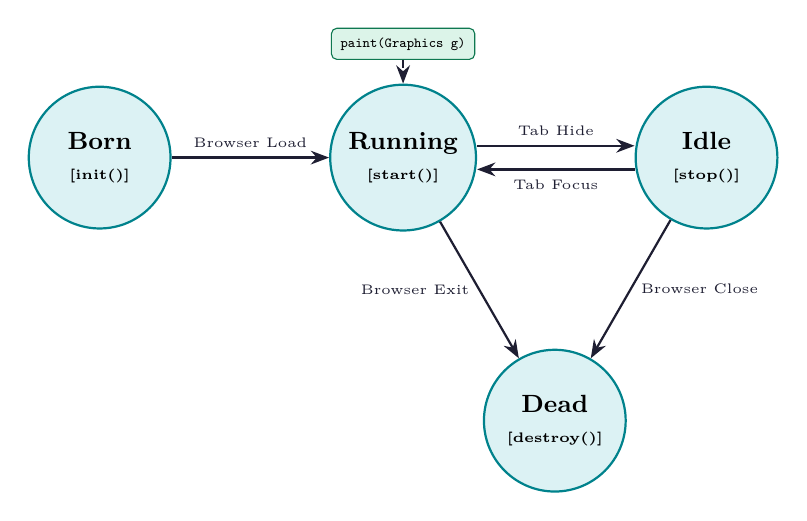
\begin{tikzpicture}[node distance=1.3cm and 1.5cm,
  state/.style={circle, draw=myteal, fill=hdrteal, minimum size=1.8cm,
    align=center, font=\small\bfseries, line width=0.8pt},
  act/.style={rectangle, draw=myamber, fill=hdramber, minimum height=0.6cm,
    font=\tiny, rounded corners=2pt, line width=0.6pt}]

  % States
  \node[state] (born) {Born\\{\tiny [init()]}};
  \node[state, right=2.0cm of born] (run) {Running\\{\tiny [start()]}};
  \node[state, right=2.0cm of run] (idle) {Idle\\{\tiny [stop()]}};
  \node[state, below=1.5cm of $(run.south)!0.5!(idle.south)$] (dead) {Dead\\{\tiny [destroy()]}};

  % Paths
  \draw[arrow] (born) -- (run) node[midway, above, font=\tiny] {Browser Load};
  \draw[arrow, transform canvas={yshift=0.15cm}] (run) -- (idle) node[midway, above, font=\tiny] {Tab Hide};
  \draw[arrow, transform canvas={yshift=-0.15cm}] (idle) -- (run) node[midway, below, font=\tiny] {Tab Focus};
  \draw[arrow] (idle) -- (dead) node[midway, right, font=\tiny] {Browser Close};
  \draw[arrow] (run) -- (dead) node[midway, left, font=\tiny] {Browser Exit};

  % Paint Call
  \node[draw=mygreen, fill=hdrgreen, rounded corners=2pt, above=0.3cm of run, font=\tiny] (pnt) {\texttt{paint(Graphics g)}};
  \draw[arrow, dashed] (pnt) -- (run);
\end{tikzpicture}
\end{tcolorbox}

\subsection{Applet Display and Status Methods}
Applets provide methods to interact with their display canvas and output messages directly to the hosting browser's status window:
\begin{itemize}[leftmargin=*, itemsep=3.5pt]
  \item \textbf{Foreground and Background Control:} Inherited from the \texttt{Component} class.
  \begin{itemize}[label=\(\circ\), leftmargin=1.5em]
    \item \texttt{void setBackground(Color c)}: Sets the background color of the applet window.
    \item \texttt{void setForeground(Color c)}: Sets the default color for text and graphical drawings inside the applet.
    \item \texttt{Color getBackground()} and \texttt{Color getForeground()}: Retrieve the current background and foreground colors.
  \end{itemize}
  \item \textbf{Status Window Output:} The browser running the applet contains a status bar (status window).
  \begin{itemize}[label=\(\circ\), leftmargin=1.5em]
    \item \texttt{void showStatus(String message)}: Displays the specified message string in the browser's status window. This is useful for user feedback (e.g., displaying coordinates, loading percentages, or event responses).
  \end{itemize}
\end{itemize}

\subsection{HTML Applet Tag and Parameters}
Applets are executed by inserting them into an HTML document using the \texttt{<applet>} tag. The browser reads the tag, downloads the compiled bytecode, and runs it inside the local JVM.

\begin{tcolorbox}[formulabox, title={\textbf{HTML <applet> Tag Syntax and Attributes}}]
\begin{verbatim}
<applet codebase="classes/" code="MyApplet.class" width="400" height="300">
    <param name="userName" value="Biraj">
    <param name="sampleRate" value="50">
    Alt text: Your browser does not support Java Applets.
</applet>
\end{verbatim}
\end{tcolorbox}

\textbf{Core attributes of the \texttt{<applet>} tag:}
\begin{itemize}[leftmargin=*, itemsep=3pt]
  \item \textbf{\texttt{code}:} Specifies the filename of the compiled applet class (mandatory).
  \item \textbf{\texttt{width} \& \texttt{height}:} Specify the initial display area dimensions in pixels (mandatory).
  \item \textbf{\texttt{codebase}:} Specifies the base URL or directory path containing the class files (optional).
  \item \textbf{\texttt{alt}:} Specifies fallback text to display if the browser supports the tag but cannot run it.
\end{itemize}

\textbf{Passing Parameters via the \texttt{<param>} Tag:}
\begin{itemize}[leftmargin=*, itemsep=3pt]
  \item Parameters are defined in HTML using the \texttt{<param name="..." value="...">} tag inside the applet block.
  \item Inside the applet's \texttt{init()} method, these parameters are retrieved as Strings using:
        \texttt{String val = getParameter("userName");}
\end{itemize}

\subsection{Applet vs. Standard Application}

\par\noindent
{\renewcommand{\arraystretch}{1.5}%
\begin{tabularx}{\linewidth}{|B{3.2cm}|Y|Y|}
\hline
\textbf{Feature} & \textbf{Applet Class} & \textbf{Standard Java Application} \\
\hline
\textbf{Execution Target} & Embedded in HTML; runs inside browser JVM. & Standalone execution on the client OS. \\
\hline
\textbf{Main Entry Method} & No \texttt{main()} entry. Uses lifecycle methods. & Requires a \texttt{public static void main} entry. \\
\hline
\textbf{Security Rules} & Heavily sandboxed (restricted access). & Full access to local hardware and file systems. \\
\hline
\textbf{Superclass Class} & Must extend \texttt{java.applet.Applet}. & Does not require a specific superclass. \\
\hline
\end{tabularx}}

% ===============================================================================
\section{Delegation Event Model}
% ===============================================================================

Java event handling is built on the \textbf{Delegation Event Model}, which separates the user interface controls from the logic handling user events.

\begin{tcolorbox}[defbox, title={\textbf{Model Components}}]
\begin{itemize}[leftmargin=*, itemsep=3pt]
  \item \textbf{Event Source:} The GUI component that generates the event when acted upon (e.g., \texttt{Button}).
  \item \textbf{Event Object:} Encapsulates details of the event state change (e.g., \texttt{ActionEvent}).
  \item \textbf{Event Listener:} An interface target that receives and processes event notifications.
\end{itemize}
\end{tcolorbox}

\begin{tcolorbox}[tikzbox, title={Delegation Event Model Architecture}]
\centering
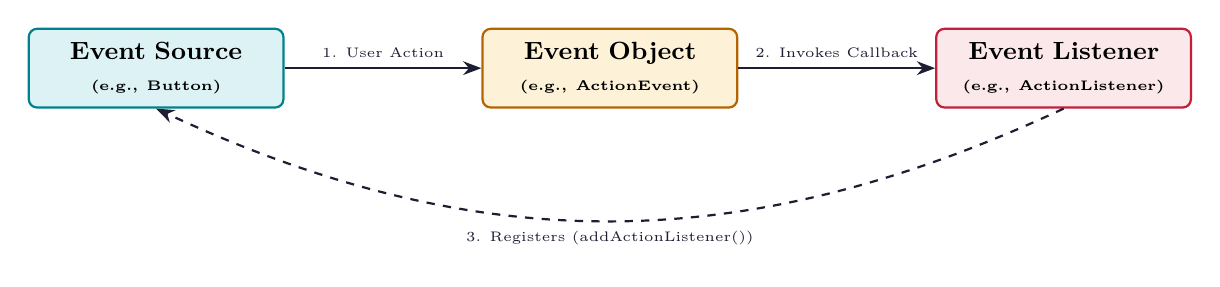
\begin{tikzpicture}[node distance=1.5cm and 2.5cm,
  source/.style={rectangle, draw=myteal, fill=hdrteal, text width=3.0cm,
    align=center, minimum height=1.0cm, font=\small\bfseries, rounded corners=3pt, line width=0.8pt},
  evt/.style={rectangle, draw=myamber, fill=hdramber, text width=3.0cm,
    align=center, minimum height=1.0cm, font=\small\bfseries, rounded corners=3pt, line width=0.8pt},
  listener/.style={rectangle, draw=myred, fill=hdrred, text width=3.0cm,
    align=center, minimum height=1.0cm, font=\small\bfseries, rounded corners=3pt, line width=0.8pt}]

  % Nodes
  \node[source] (src) {Event Source\\{\tiny (e.g., Button)}};
  \node[evt, right=of src] (obj) {Event Object\\{\tiny (e.g., ActionEvent)}};
  \node[listener, right=of obj] (lis) {Event Listener\\{\tiny (e.g., ActionListener)}};

  % Paths
  \draw[arrow] (src) -- (obj) node[midway, above, font=\tiny] {1. User Action};
  \draw[arrow] (obj) -- (lis) node[midway, above, font=\tiny] {2. Invokes Callback};
  
  % Registration path
  \draw[arrow, dashed, bend left=25] (lis.south) to node[midway, below, font=\tiny] {3. Registers (addActionListener())} (src.south);
\end{tikzpicture}
\end{tcolorbox}

\subsection{Adapter Classes}
An event listener interface may define multiple abstract methods (e.g., \texttt{WindowListener} defines seven). Implementing it directly forces you to provide empty overrides for all of them.

\begin{tcolorbox}[defbox, title={\textbf{Adapter Class Solution}}]
An \textbf{Adapter Class} is a helper class that implements a listener interface with empty default method overrides. By extending the adapter class (e.g., extending \texttt{WindowAdapter}), you only override the specific callback methods you need.
\tcbset{after={\color{black}}}
\end{tcolorbox}

% ===============================================================================
\section{AWT (Abstract Window Toolkit)}
% ===============================================================================

AWT is Java's original platform-dependent GUI library. It uses native system peers to render controls, resulting in a look-and-feel that matches the host OS.

\begin{tcolorbox}[tikzbox, title={AWT Component Class Hierarchy}]
\centering
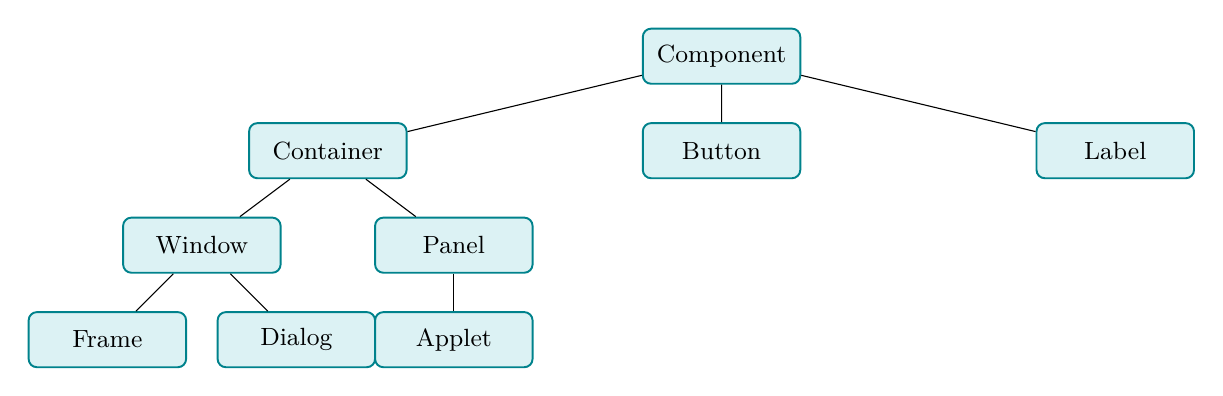
\begin{tikzpicture}[
  level 1/.style={sibling distance=5cm, level distance=1.2cm},
  level 2/.style={sibling distance=3.2cm, level distance=1.2cm},
  level 3/.style={sibling distance=2.4cm, level distance=1.2cm},
  node/.style={rectangle, draw=myteal, fill=hdrteal, minimum height=0.7cm, minimum width=2.0cm, font=\small, rounded corners=3pt, align=center, line width=0.7pt}
]
  \node[node] {Component}
    child { node[node] {Container}
      child { node[node] {Window}
        child { node[node] {Frame} }
        child { node[node] {Dialog} }
      }
      child { node[node] {Panel}
        child { node[node] {Applet} }
      }
    }
    child { node[node] {Button} }
    child { node[node] {Label} };
\end{tikzpicture}
\end{tcolorbox}

\subsection{AWT vs. Swing}

\par\noindent
{\renewcommand{\arraystretch}{1.5}%
\begin{tabularx}{\linewidth}{|B{3.2cm}|Y|Y|}
\hline
\textbf{Metric} & \textbf{AWT (Heavyweight)} & \textbf{Swing (Lightweight)} \\
\hline
\textbf{Rendering Engine} & Uses host OS peer components. & Rendered purely in Java (custom painting). \\
\hline
\textbf{Platform Style} & Platform-dependent look-and-feel. & Platform-independent look-and-feel. \\
\hline
\textbf{Speed} & Fast (delegates rendering to host). & Slower (rendered by JVM engine). \\
\hline
\textbf{Class Package} & Lives in \texttt{java.awt.*} & Lives in \texttt{javax.swing.*} \\
\hline
\end{tabularx}}

\subsection{Layout Managers}
Layout managers control the sizing and positioning of child components inside a container:
\begin{itemize}[leftmargin=*, itemsep=3pt]
  \item \textbf{FlowLayout (Default for Panel/Applet):} Places components in a row, wrapping when the boundary is reached.
  \item \textbf{BorderLayout (Default for Frame/Window):} Places components in five regions: North, South, East, West, Center.
  \item \textbf{GridLayout:} Places components in a uniform grid of equal-sized rows and columns.
\end{itemize}

\newpage
% ===============================================================================
\begin{center}
  {\large\bfseries\color{myred} Quick Revision --- Module 5}\\[3pt]
  {\small\color{mydark} Applets, Event Handling \& AWT Controls $|$ OE-EC704A}
\end{center}
\noindent{\color{myred}\rule{\linewidth}{1.2pt}}
\vspace{4pt}

\begin{tcolorbox}[formulabox, title={\textbf{HTML Applet \& Event Handling Syntax}}]
{\renewcommand{\arraystretch}{1.3}%
\begin{tabularx}{\linewidth}{l Y}
\textbf{Concept} & \textbf{Syntax and Example Usage} \\
\hline
HTML Applet Tag & \texttt{<applet code="MyApplet.class" width="300" height="200"></applet>} \\
Applet Parameters & \texttt{<param name="message" value="Hello World">} \\
Parameter Query & \texttt{String val = getParameter("message");} \\
Applet paint Override & \texttt{public void paint(Graphics g) \{ g.drawString("Test", 20, 20); \}} \\
\hline
\textbf{AWT \& Events} & \textbf{Registration \& Design Declarations} \\
\hline
AWT Button Registration & \texttt{Button btn = new Button("Submit"); btn.addActionListener(listener);} \\
Anonymous Inner Class & \texttt{btn.addActionListener(new ActionListener() \{ ... \});} \\
Set Frame Layout & \texttt{setLayout(new BorderLayout()); add(btn, BorderLayout.NORTH);} \\
AWT Frame Show & \texttt{Frame f = new Frame("Title"); f.setSize(300, 300); f.setVisible(true);} \\
\end{tabularx}}
\end{tcolorbox}

\begin{tcolorbox}[defbox, title={\textbf{One-Line Definitions}}]
\begin{itemize}[leftmargin=*, itemsep=2pt]
  \item \textbf{Applet:} A small Java program executed inside a web browser container.
  \item \textbf{Delegation Event Model:} An event framework separating event detection from handler logic.
  \item \textbf{Event Source:} A UI component that registers listeners and fires events on state changes.
  \item \textbf{Event Listener:} An interface declaring callback methods to handle specific events.
  \item \textbf{Adapter Class:} A helper class with default empty implementations of a listener interface.
  \item \textbf{Anonymous Inner Class:} An unnamed inline class used to implement listener interfaces.
  \item \textbf{AWT:} A platform-dependent GUI library utilizing host OS peers for rendering.
  \item \textbf{Layout Manager:} A layout interface deciding the spatial distribution of child components.
\end{itemize}
\tcbset{after={\color{black}}}
\end{tcolorbox}

\begin{tcolorbox}[exambox, title={\textbf{Frequently Asked / Viva Questions}}]
\begin{enumerate}[leftmargin=*, label=\textbf{Q\arabic*.}, itemsep=5pt]
  \item \Q{Which class does every Java Applet extend? Which package contains it?}
        Every Applet extends \texttt{java.applet.Applet} (or \texttt{javax.swing.JApplet} for Swing). The class resides inside the \texttt{java.applet} package.
        
  \item \Q{Why does an applet not contain a \texttt{main()} method?}
        Applets do not run as standalone applications. They are executed by a web browser container, which handles loading and calls their lifecycle methods.
        
  \item \Q{What is the difference between \texttt{init()} and \texttt{start()} methods?}
        \texttt{init()} is called once when the applet is first loaded to handle initialization. \texttt{start()} is called every time the user visits or returns to the page.
        
  \item \Q{What is the purpose of the \texttt{paint(Graphics g)} method? Who calls it?}
        The \texttt{paint()} method renders the applet graphics (text, lines, shapes) on the screen. It is called by the browser JVM when the applet first displays or needs redrawing.
        
  \item \Q{How do you pass parameters from HTML to an Applet?}
        Using the \texttt{<param>} tag inside the \texttt{<applet>} tag in HTML, and querying it in the applet using the \texttt{getParameter(String name)} method.
        
  \item \Q{What is the difference between \texttt{getCodeBase()} and \texttt{getDocumentBase()}?}
        \texttt{getCodeBase()} returns the URL of the directory containing the applet's compiled class files. \texttt{getDocumentBase()} returns the URL of the HTML document embedding the applet.
        
  \item \Q{Why are AWT components referred to as heavyweight controls?}
        AWT controls are coupled to the underlying operating system. Each AWT component is associated with a native peer window, consuming significant memory and OS resources.
        
  \item \Q{What is the purpose of an Adapter class in event handling?}
        It simplifies listener implementation. By extending an adapter class, you only override the specific event handler methods you need, rather than providing empty overrides for all methods.
        
  \item \Q{How does FlowLayout arrange components? What is its default alignment?}
        FlowLayout arranges components in a single line from left to right. When it runs out of space, it wraps them to the next line. Its default alignment is centered.
        
  \item \Q{Why did AWT become deprecated in favor of Swing?}
        AWT's platform-dependent rendering led to inconsistent layouts across operating systems. Swing introduced lightweight, platform-independent controls rendered entirely in Java.
\end{enumerate}
\end{tcolorbox}

\begin{tcolorbox}[tikzbox, title={Applet Lifecycle Methods Transition Matrix}]
\centering
{\renewcommand{\arraystretch}{1.45}%
\begin{tabularx}{\linewidth}{|B{3.0cm}|Y|Y|}
\hline
\textbf{Method} & \textbf{Invocation Frequency} & \textbf{Primary Purpose} \\
\hline
\textbf{\texttt{init()}} & Invoked once when first loaded. & Initializes variables, loads fonts, images, and GUI elements. \\
\hline
\textbf{\texttt{start()}} & Invoked on load and page returns. & Resumes applet execution, starts animations or threads. \\
\hline
\textbf{\texttt{paint()}} & Invoked on display and redraw requests. & Renders text, shapes, and images to the screen coordinate system. \\
\hline
\textbf{\texttt{stop()}} & Invoked on page exit or tab switch. & Suspends threads, pauses animations to save CPU resources. \\
\hline
\textbf{\texttt{destroy()}} & Invoked once before unloading. & Reclaims resources, kills threads, and cleans up memory. \\
\hline
\end{tabularx}}
\end{tcolorbox}

\end{document}
